\section{Introduction}

Software packages are widely used in software development to improve productivity. Usage of software packages is complicated by \emph{package versioning}, \emph{transitive dependency} and \emph{complex dependency constraints}.


\subsection{The Dependency Management Problem}

Software packages evolve over time, some supported features might not longer be supported afterwards, some interface might be changed or deprecated later. Software packages are usually versioned by some \emph{versionning scheme} to clearly mark the changes in each version. Users of a package should know the exact version that's been used to make sure it supports all the required features and the documentation conforms to the specific version.

Software package dependency is transitive. If x depends on y, and y depends on z, then x depends on z. Though developers usually only specify the direct dependencies as a flat list, it expands to a complex directed graph in most cases.

Software dependency management requires the support of complex constraints, like \emph{fuzzy version constraints}, \emph{excludes in transitive dependency}, \emph{intransitive dependency}, etc. For example, in both Ivy and Maven, it's possible to specify fuzzy version constraints, such as $(, 1.0.0]$, $[1.5.2, 1.6.0)$, etc, or to exclude a specific package from all later transitive dependencies. In Ivy, it's possible to mark a dependency as intransitive.

Generally, there're two common problems related to software dependency management -- one is \emph{conflicts}, the other is \emph{missing dependency}. Usually, only one version of a package can be used in the same project. If a project depends on two different versions of the same package, then there's a \emph{conflict}. On the other hand, if a project depends on a package that can't be found, then there's a \emph{missing dependency}.

The complexity of software packages necessitates tools to automatically check whether a dependency specification can be satisfied or not. More concretely, a dependency manager has to check that for a given dependency specification (1) whether there exists conflicts or missing dependencies; (2) if there's no error, generate an optimal set of packages so that the dependency constraints of the specification and of each package are satisfied.


\subsection{The Need for a New Dependency Resolution Algorithm}

In the Java world, Maven and Ivy are the most widely used dependency management tools. In Scala, SBT depends on Ivy to resolve dependencies.

The common problem with Ivy and Maven is that they resort to conflict managers unnecessarily even when the specification is satisfiable with no conflicts. This is better illustrated with Figure \ref{fig:introuction:underconstraint}, where the rectangles represents versioned packages, and the rounded rectangles represent dependency constraints.  As we can see in the graph, the project depends on the package A and B directly, and they in turn depend on the package C.

It's obvious that the dependency graph in Figure \ref{fig:introuction:underconstraint} has a solution set $\{(A, 3.5), (B, 1.2), (C, 2.4)\}$. However, both Maven and Ivy would think there's a conflict on the package $C$, and the conflict manager would be called to resolve the conflict. Depending on the setting of the conflict manager, usually $(C, 2.5)$ will be chosen, which is incorrect!

Ivy and Maven fail in such cases because no backtracking is tried at all when conflict happens, instead they always resort to conflict managers.

\begin{figure}[ht]
  \center
  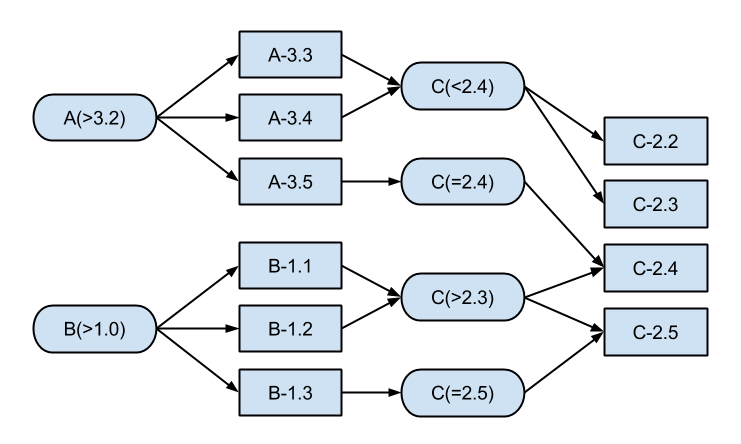
\includegraphics[width=14cm]{img/introduction/underconstraint.png}
  \caption[An example dependency graph]{An example dependency graph \label{fig:introuction:underconstraint}}
\end{figure}

In this report, I'll describe in detail how to implement a dependency management algorithm based on SAT solvers, which overcomes the drawbacks of Maven and Ivy. I'll also discuss some general reflections about software dependency management, which might be helpful for future ecosystem designers.

%% \subsection{Maven Ecosystem}

%% - scopes
%% - excludes

%% \subsection{Ivy Ecosystem}

%% - configuration
%% - module
%% - artifacts
%% - force
%% - transitive
